\documentclass[
  12pt,
  openright,
  twoside,
  a4paper,
  english,
  french,
  spanish,
  brazil
]{abntex2}

\usepackage{lmodern}
\usepackage[T1]{fontenc}
\usepackage[utf8]{inputenc}
\usepackage{indentfirst}
\usepackage{color}
\usepackage{graphicx}
\usepackage{microtype}
\usepackage[brazilian,hyperpageref]{backref}
\usepackage{abntex2cite}
\usepackage{customization}
\usepackage{hyperref}

\renewcommand{\backrefpagesname}{Citado na(s) página(s):~}
\renewcommand{\backref}{}
\renewcommand*{\backrefalt}[4]{
	\ifcase #1
		Nenhuma citação no texto.
	\or
		Citado na página #2.
	\else
		Citado #1 vezes nas páginas #2.
	\fi
}

\titulo{Guia de Acessibilidade Digital}
\autor{Grupo 06}
\local{Brasília, Brasil}
\data{2024, v1.6.0}
\orientador{Rejane Figueiredo}
\instituicao{
  Universidade de Brasília
  \par
  Faculdade do Gama
}
\tipotrabalho{Relatório técnico}
\preambulo{
  Trabalho submetido à disciplina de Interação Humano-Computador da Universidade
  de Brasília, ministrada pela professora Rejane Figueiredo.
}

\definecolor{blue}{RGB}{41,5,195}

\makeatletter
\hypersetup{
  pdftitle={\@title},
  pdfauthor={\@author},
  pdfsubject={\imprimirpreambulo},
  pdfcreator={LaTeX with abnTeX2},
  pdfkeywords={abnt}{latex}{abntex}{abntex2}{trabalho acadêmico},
  colorlinks=true,
  linkcolor=blue,
  citecolor=blue,
  filecolor=magenta,
  urlcolor=blue,
  bookmarksdepth=4
}
\makeatother

\makeatletter
\setlength{\@fptop}{5pt}
\makeatother

\newcommand{\quadroname}{Quadro}
\newcommand{\listofquadrosname}{Lista de quadros}

\newfloat[chapter]{quadro}{loq}{\quadroname}
\newlistof{listofquadros}{loq}{\listofquadrosname}
\newlistentry{quadro}{loq}{0}

\setfloatadjustment{quadro}{\centering}
\counterwithout{quadro}{chapter}
\renewcommand{\cftquadroname}{\quadroname\space}
\renewcommand*{\cftquadroaftersnum}{\hfill--\hfill}

\setfloatlocations{quadro}{hbtp}

\setlength{\parindent}{1.3cm}
\setlength{\parskip}{0.2cm}

\makeindex

\begin{document}

\selectlanguage{brazil}
\frenchspacing

\pretextual
\imprimircapa
\imprimirfolhaderosto*

\begin{agradecimentos}
  Os agradecimentos principais são direcionados à professora Rejane Figueiredo,
  que ministrou a disciplina de Interação Humano-Computador. Sua dedicação e
  paciência foram fundamentais para o desenvolvimento deste guia.
\end{agradecimentos}

% ---
% RESUMOS
% ---

% resumo em português
\setlength{\absparsep}{18pt} % ajusta o espaçamento dos parágrafos do resumo
\begin{resumo}
 Segundo a \citeonline[3.1-3.2]{NBR6028:2003}, o resumo deve ressaltar o
 objetivo, o método, os resultados e as conclusões do documento. A ordem e a extensão
 destes itens dependem do tipo de resumo (informativo ou indicativo) e do
 tratamento que cada item recebe no documento original. O resumo deve ser
 precedido da referência do documento, com exceção do resumo inserido no
 próprio documento. (\ldots) As palavras-chave devem figurar logo abaixo do
 resumo, antecedidas da expressão Palavras-chave:, separadas entre si por
 ponto e finalizadas também por ponto.

  \textbf{Palavras-chave}:
  Interação Humano-Computador. Guia de acessibilidade digital. Design de
  serviços. Pessoas com deficiência. Tecnologia da informação. Experiência do
  usuário. Acessibilidade.
\end{resumo}

\cleardoublepage

\begin{siglas}
  \item[ASES] Avaliador e Simulador de Acessibilidade em Sítios
  \item[CSS] \textit{Cascading Style Sheets}
  \item[DADI] \textit{Definition Architecture Design Implementation}
  \item[DCU] Design Centrado no Usuário
  \item[DOM] \textit{Document Object Model}
  \item[eMAG] Modelo de Acessibilidade em Governo Eletrônico
  \item[ePWG] Padrões Web em Governo Eletrônico
  \item[GOMS] \textit{Goals, Operators, Methods, and Selection rules}
  \item[HTML] \textit{HyperText Markup Language}
  \item[IBGE] Instituto Brasileiro de Geografia e Estatística
  \item[IHC] Interação Humano-Computador
  \item[PCD] Pessoas com Deficiência
  \item[TI] Tecnologia da Informação
  \item[TIC] Tecnologias de Informação e Comunicação
  \item[UX] \textit{User Experience}
  \item[W3C] \textit{World Wide Web Consortium}
  \item[WAI] \textit{Web Accessibility Initiative}
  \item[WAI-ARIA]
    \textit{
      Web Accessibility Initiative - Accessible Rich Internet Applications
    }
  \item[WCAG] \textit{Web Content Accessibility Guidelines}
  \item[XHTML] \textit{eXtensible HyperText Markup Language}
  \item[XML] \textit{eXtensible Markup Language}
  % \item[DS] Design de Serviços
  % \item[ISO] \textit{International Organization for Standardization}
  % \item[IHIP] \textit{Intangible, Heterogeneous, Inseparable and Perishable}
\end{siglas}

\pdfbookmark[0]{\contentsname}{toc}
\tableofcontents*
\cleardoublepage

\textual

\chapter{Introdução}

Este guia de acessibilidade digital foi criado como resultado da disciplina de
IHC da Faculdade do Gama da Universidade de Brasília, com o intuito de aplicar e
demonstrar os conhecimentos dos estudantes do grupo sobre os conteúdos
apresentados na disciplina durante o primeiro semestre de 2024.

O objetivo é oferecer a todo profissional da área de TI subsídios teóricos e
práticos, tanto no âmbito documental e ferramental, para que o desenvolvedor
possa compreender os conceitos sobre IHC e aplique estratégias de transformação
digital acessível, considerando que o sistema a ser desenvolvido será adequado à
PCDs e implemente a estrutura de acessibilidade definida pelo Governo Federal.

Esse material se faz de grande importância para manter os conhecimentos
``frescos'' sobre acessibilidade na web, seja para o profissional que não
conhece o tema ter a oportunidade de estudá-lo, como para o mais experiente
consultar informações técnicas.

A acessibilidade digital importa pois, de acordo com números fornecidos pelo
IBGE, mais de 45 milhões de cidadãos brasileiros possuem alguma deficiência
\cite{DAP:Guia-de-Boas-Praticas}. Dificuldades para interagir e compreender o
conteúdo de uma aplicação web, não conseguir concluir cadastros ou pagamentos e
falta de botões acessíveis podem se tornar um grande empecilho ao indivíduo.

Quando conteúdos presentes na internet, em aplicativos para telefone, vídeos nas
plataformas digitais e conteúdos televisivos são acessíveis, todas as pessoas
são beneficiadas, especialmente as que possuem algum tipo de deficiência,
oferecendo conforto e segurança a este público-alvo.

As diretrizes do WCAG do W3C oferecem um caminho acessível à web, com a
acessibilidade sendo tratada em três grandes pontos: design, conteúdo e
desenvolvimento. O conceito de \textit{device-agnostic} é o qual o WCAG se
baseia, o que significa que a s recomendações se referem, com contrastes e
botões sendo acessíveis tanto no computador, como nos aparelhos móveis
\cite{DAP:Guia-de-Boas-Praticas}.

Ao final desta etapa, espera-se do profissional de TI que:

\begin{itemize}
  \item conheça a necessidade de ser acessível na contemporaneidade;
  \item identifique a importância do material para consultas do time de TI; e
  \item
    compreenda o impacto que introduzir acessibilidade no cotidiano do
    desenvolvimento pode acarretar na população.
\end{itemize}

\chapter{IHC Não é Engenharia de Software, Mas...}

\section{Abordagens Teóricas em IHC}

A Interação Humano-Computador (IHC) é uma área interdisciplinar que foca no
design, avaliação e implementação de sistemas computacionais interativos com
ênfase nas interfaces entre usuários humanos e computadores. O objetivo é
melhorar a usabilidade e a experiência do usuário, tornando os sistemas mais
eficientes e intuitivos.

Diferentes abordagens teóricas em IHC buscam entender e melhorar essa interação,
essas abordagens teóricas servem como bússolas, guiando o design e a avaliação
de sistemas que conectam pessoas e tecnologias. Aprofundando nessas abordagens,
desvendamos os princípios que fundamentam a criação de interfaces intuitivas,
eficientes e agradáveis.

\begin{itemize}
  \item \textbf{Psicologia Cognitiva}

    A psicologia cognitiva é um pilar fundamental na IHC, explorando os
    mecanismos internos da mente humana que moldam a forma como interagimos com
    computadores. Essa abordagem é crucial para entender como as pessoas
    processam informações e como os sistemas computacionais podem ser projetados
    para apoiar esses processos. Modelos como o GOMS (Goals, Operators, Methods,
    and Selection rules) ajudam a prever o desempenho do usuário.

  \item \textbf{Etnografia}

    A etnografia envolve a observação e descrição detalhada das atividades dos
    usuários em seus contextos naturais. Através dessa observação podemos
    desvendar seus comportamentos, necessidades e motivações, contextualizando a
    interação com a tecnologia. Isso ajuda a entender como a tecnologia é
    realmente usada e pode revelar problemas e oportunidades que não seriam
    visíveis através de outros métodos.

  % Para evitar um overbox nessa parte, foi necessário quebrar a lista em duas
  % partes.
  \newpage

  \item \textbf{Design Centrado no Usuário (DCU)}

    O DCU destaca-se como uma filosofia de design que coloca as necessidades,
    desejos e expectativas dos usuários no centro do processo de
    desenvolvimento. Através de métodos como entrevistas, questionários e testes
    de usabilidade, podemos obter feedbacks valiosos dos usuários e moldar o
    sistema de acordo com suas expectativas e demandas.
\end{itemize}

\section{Processos de Design de IHC}

Os processos de design de IHC são estruturados para criar interfaces que sejam
eficientes, eficazes e agradáveis para os usuários. Os principais processos são:

\begin{enumerate}
  \item Pesquisa e Análise de Usuários
  \begin{itemize}
    \item
      Entendimento do Contexto de Uso: compreender o ambiente e as condições de
      uso da aplicação.
    \item
      Perfis de Usuários (Personas): criar representações dos diferentes tipos
      de usuários.
    \item
      Análise de Tarefas: identificar e detalhar as tarefas que os usuários
      precisam realizar.
  \end{itemize}
  \item Requisitos e Especificações
  \begin{itemize}
    \item Requisitos Funcionais: definir o que a aplicação deve fazer.
    \item
      Requisitos Não-Funcionais: definir como a aplicação deve se comportar,
      considerando usabilidade, acessibilidade, etc.
    \item
      Requisitos de Usuário: identificar as necessidades e expectativas dos
      usuários.
  \end{itemize}
  \item Design de Interface
  \begin{itemize}
    \item
      Sketches e Wireframes: criar desenhos iniciais para mostrar a estrutura
      básica da interface gráfica.
    \item
      Protótipos de Baixa Fidelidade: desenvolver protótipos simples para testes
      iniciais.
    \item
      Protótipos de Alta Fidelidade: criar protótipos interativos e detalhados,
      próximos do produto final.
  \end{itemize}
  \item Avaliação e Testes
  \begin{itemize}
    \item
      Testes de Usabilidade: realizar testes com usuários reais para identificar
      problemas.
    \item
      Avaliações Heurísticas: especialistas em usabilidade avaliam a interface
      com base em heurísticas.
    \item Feedback dos Usuários: coletar opiniões e sugestões dos usuários.
  \end{itemize}
  \item Implementação
  \begin{itemize}
    \item Desenvolvimento: programar a interface conforme o design especificado.
    \item Integração: integrar a interface com outros sistemas e componentes.
  \end{itemize}
  \item Lançamento e Manutenção
  \begin{itemize}
    \item \textit{Deploy}: lançar a interface para os usuários finais.
    \item
      Monitoramento: acompanhar o uso da interface e coletar dados de desempenho
      e usabilidade.
    \item
      Atualizações: melhorar e corrigir a interface com base no feedback dos
      usuários e nas métricas coletadas.
  \end{itemize}
  \item Metodologias e Abordagens
  \begin{itemize}
    \item
      Design Centrado no Usuário (DCU): foco principal nas necessidades e
      características dos usuários.
    \item
      \textit{Design Thinking}: processo iterativo que envolve empatia,
      definição de problemas, ideação, prototipagem e teste.
    \item
      Métodos Ágeis: iterações curtas de design e desenvolvimento com feedback
      contínuo dos usuários.
  \end{itemize}
\end{enumerate}

Essas etapas são frequentemente iterativas, permitindo ajustes e refinamentos
contínuos para garantir uma experiência de usuário de alta qualidade,
satisfazendo suas necessidades e expectativas.

\section{Identificação de Necessidades dos Usuários}

Identificar as necessidades dos usuários é uma parte fundamental no processo de
design de IHC. É um processo que visa entender as reais necessidades,
expectativas e problemas enfrentados pelos usuários, e somente após essa
compreensão desenvolver interfaces que atendam efetivamente a essas demandas. Os
principais métodos para identificar as necessidades dos usuários são:

\begin{enumerate}
  \item Entrevistas
  \begin{itemize}
    \item
      Entrevistas Estruturadas: perguntas pré-definidas para obter informações
      específicas.
    \item
      Entrevistas Não-Estruturadas: conversas livres para explorar profundamente
      os pensamentos e sentimentos dos usuários.
  \end{itemize}
  \item Observação
  \begin{itemize}
    \item
      Observação Direta: assistir os usuários enquanto eles interagem com o
      sistema ou realizam tarefas em seu ambiente natural.
    \item
      Etnografia: imersão no ambiente dos usuários para entender o contexto e as
      práticas cotidianas.
  \end{itemize}
  \item Questionários e Pesquisas
  \begin{itemize}
    \item
      Questionários: coletar dados quantitativos e qualitativos através de
      perguntas fechadas e abertas.
    \item
      Pesquisas Online: distribuir questionários amplamente para alcançar um
      grande número de usuários.
  \end{itemize}
  \item Estudos de Usabilidade
  \begin{itemize}
    \item
      Testes de Usabilidade: observar os usuários enquanto eles tentam completar
      tarefas específicas com o sistema.
    \item
      Feedback Pós-Tarefa: coletar feedback imediato dos usuários após a
      realização de tarefas.
  \end{itemize}
  \item Personas e Cenários
  \begin{itemize}
    \item
      Criação de Personas: desenvolver perfis fictícios de usuários baseados em
      dados reais para representar diferentes tipos de usuários.
    \item
      Desenvolvimento de Cenários: criar histórias que descrevem como os
      usuários interagem com o sistema em diferentes situações.
  \end{itemize}
\end{enumerate}

A combinação desses métodos ajuda a criar um entendimento abrangente das
necessidades dos usuários, garantindo que o design final seja relevante e
eficaz.

\section{Jornada do Usuário} \label{user-journey}

É uma sequência de passos necessários que o usuário deve realizar para completar
um objetivo com uma empresa ou produto, geralmente mostrado em relação ao tempo
(do primeiro contato até a fidelização) ou em relação aos canais. Esta jornada
inclui todas as etapas, interações e emoções que o usuário experimenta ao longo
do caminho. O objetivo de mapear a jornada do usuário é entender melhor as
necessidades, expectativas e possíveis frustrações do usuário, para melhorar a
experiência e a satisfação geral.

Entenda canais como as diferentes fontes de comunicação e/ou origens de
informação que o usuário pode usar para se comunicar com o produto ou com a
empresa.

Vamos citar um exemplo prático. Na compra de um livro pela internet, as etapas
da jornada do usuário incluem:

\begin{enumerate}
  \item Descoberta do livro
  \item Pesquisa do livro em diferentes sites
  \item Comparação de preço
  \item Leitura das avaliações de outros usuários
  \item Compra
  \item Recebimento do produto
  \item Leitura do livro
  \item Feedback e fidelização
\end{enumerate}

Desse jeito, podemos mapear a jornada do usuário da seguinte forma:

\begin{itemize}
  \item Definir o objetivo do usuário
  \item Identificar as etapas da jornada
  \item Mapear os pontos de interação
  \item Identificar pontos de melhoria
  \item Desenhar o mapa da jornada do usuário
\end{itemize}

Exemplos de ferramentas para mapear a jornada do usuário são:

\begin{enumerate}
  \item
    Figma: utilizado para design de interfaces e prototipagem, permite a criação
    de \textit{wireframes} e protótipos interativos.
  \item
    Miro: ideal para \textit{brainstorming}, mapeamento de jornada e diagramas.
  \item
    Sketch: ferramenta de design digital focada em criação de interfaces,
    oferece integração com diversos plugins para UX.
  \item
    Lucidchart: ferramenta para criação de diagramas e mapas de processos, útil
    para mapear visualmente a jornada do usuário.
\end{enumerate}

\section{Fluxo do Usuário}

É um conjunto de instruções ou de interações necessárias que descrevem um
conjunto ideal de passos que o usuário deve realizar para executar uma tarefa
específica com um produto. O fluxo de usuário detalha cada passo que o usuário
dá, desde a entrada inicial até a conclusão da tarefa, mostrando as escolhas,
ações e feedbacks ao longo do caminho.

O objetivo do fluxo do usuário é garantir que a experiência seja intuitiva,
eficiente e sem obstáculos, facilitando a realização das metas do usuário. Esse
conceito é fundamental em design de UX e desenvolvimento de produtos digitais.

Seguindo o exemplo do tópico anterior (\ref{user-journey}) na compra de um livro
pela internet, as etapas do fluxo do usuário incluem:

\begin{enumerate}
  \item Descoberta do Livro
  \begin{itemize}
    \item
      Ação: o usuário descobre um livro através de redes sociais ou através da
      recomendação de um amigo.
  \end{itemize}
  \item Pesquisa do Livro em Diferentes Sites
  \begin{itemize}
    \item
      Ação: o usuário pesquisa o título do livro e visita diferentes sites de
      livrarias online.
  \end{itemize}
  \item Comparação de Preço
  \begin{itemize}
    \item Ação: o usuário compara preços do livro em várias livrarias online.
    \item
      Possíveis Frustrações: diferenças de preço significativas e custos de
      envio altos.
  \end{itemize}
  \item Leitura das Avaliações de Outros Usuários
  \begin{itemize}
    \item
      Ação: o usuário lê avaliações e comentários de outros leitores para
      avaliar a qualidade do livro.
    \item
      Possíveis Frustrações: avaliações contraditórias ou ausência de avaliações
      suficientes.
  \end{itemize}
  \item Compra
  \begin{itemize}
    \item
      Ação: o usuário adiciona o livro ao carrinho, insere as informações de
      pagamento e finaliza a compra.
    \item
      Possíveis Frustrações: problemas de pagamento ou falta de opções de
      pagamento.
  \end{itemize}
  \item Recebimento do Produto
  \begin{itemize}
    \item Ação: o usuário recebe o livro em casa.
    \item
      Possíveis Frustrações: atrasos na entrega ou estado danificado do produto.
  \end{itemize}
  \item Leitura do Livro
  \begin{itemize}
    \item Ação: o usuário lê o livro.
    \item
      Possíveis Frustrações: qualidade do produto não corresponder às
      expectativas.
  \end{itemize}
  \item Feedback e Fidelização
  \begin{itemize}
    \item
      Ação: o usuário deixa uma avaliação do livro e possivelmente segue a loja
      da livraria nas redes sociais.
  \end{itemize}
\end{enumerate}

As mesmas ferramentas citadas no tópico anterior (\ref{user-journey}) também
servem para realizar o mapeamento do fluxo do usuário.

\section{Mapa de Jornada}

Um mapa de jornada é uma visualização do processo que uma pessoa passa com o
intuito de cumprir um determinado objetivo. Em sua forma mais básica, começa
compilando uma série de ações do usuário dentro de uma linha do tempo. Em
seguida, a linha do tempo é desenvolvida com pensamentos e emoções do usuário a
fim de criar uma narrativa. Essa narrativa é condensada e polida, levando a uma
visualização.

Esse tipo de modelo é dividido em três seções verticais: o topo mostra a
persona, um cenário e um objetivo específico, o meio mostra fases de alto nível
que compreendem ações, pensamentos, emoções do usuário, e o final mostra as
conclusões, \textit{insights} e propriedades internas daquele mapa.

\section{Ponto de Serviço}

O ponto de serviço é focado para visualizar as relações entre componentes
diferentes de serviços (como pessoas, negócios ou processos) em diversos pontos
de contato em uma jornada específica de um cliente. Você pode enxergar um mapa
de jornada como um mapa turístico de uma cidade, mostrando a rota do turista e
destacando pontos de interesse. Em contrapartida, o ponto de serviço seria um
mapa da cidade da perspectiva de um planejador urbano, mostrando o layout de
ruas, edifícios e infraestrutura. Mapas de jornada são melhores para entender a
experiência do usuário, enquanto planos de serviço são melhores para documentar
e aprimorar processos de serviço.

\begin{figure}[htb]
  \caption{\label{service-blueprint} Exemplo de ponto de serviço}
  \begin{center}
    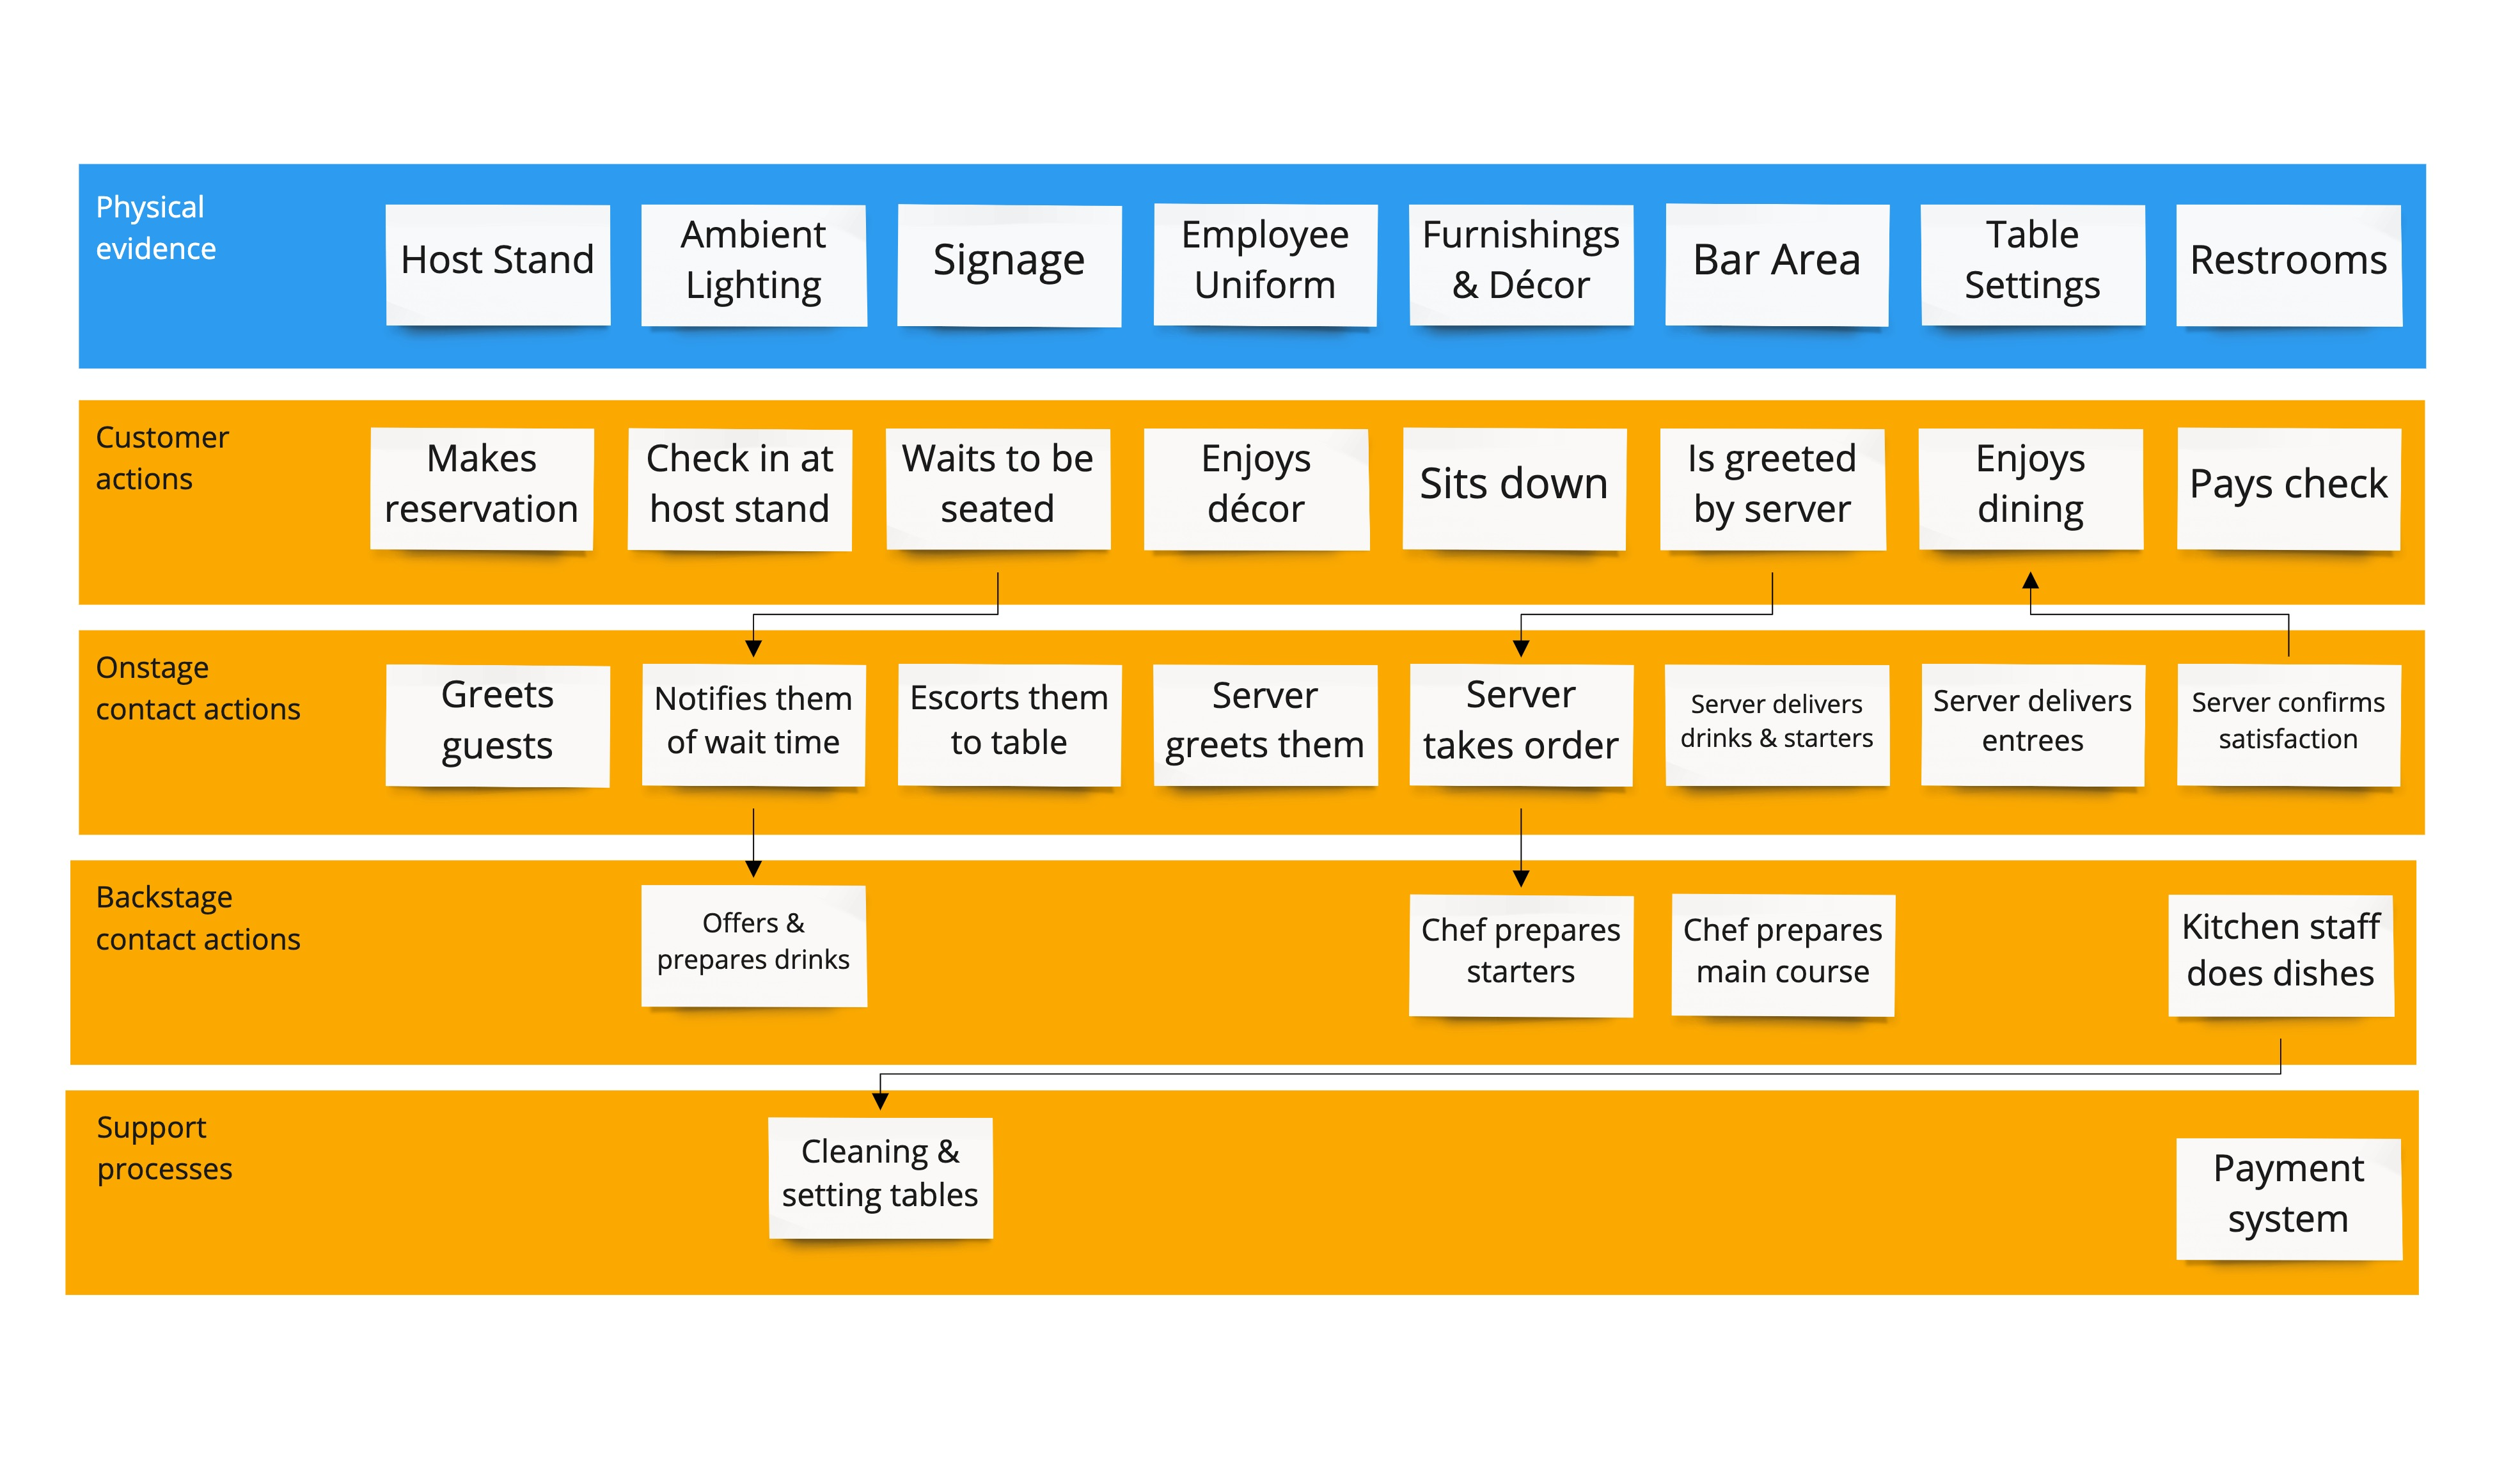
\includegraphics[width=0.85\textwidth]{assets/service-blueprint.png}
  \end{center}
  \legend{Fonte: Página do Miro \cite{Miro:Service-Blueprints}}
\end{figure}

% Para evitar que o quadro fique na página seguinte, foi necessário quebrar a
% página.
\newpage

\section{Mapa de História do Usuário}

\chapter{Modelo de Acessibilidade}

O Modelo de Acessibilidade em Governo Eletrônico (eMAG) consiste em um conjunto
de recomendações a ser considerado para que o processo de acessibilidade dos
sites e portais do governo brasileiro seja conduzido de forma padronizada e de
fácil implementação. Ele é coerente com as necessidades brasileiras e em
conformidade com os padrões internacionais, sendo formulado para orientar
profissionais que tenham contato com publicação de informações ou serviços na
internet a desenvolver, alterar e/ou adequar páginas, sites e portais,
tornando-os acessíveis ao maior número de pessoas possível.

\section{O Acesso de Pessoas com Deficiência}

Quatro principais situações vivenciadas por usuários com deficiência são:

\begin{enumerate}
  \item
    acesso ao computador sem o mouse (pessoas com deficiência visual,
    dificuldade de controle dos movimentos, paralisia ou amputação de um membro
    superior);
  \item
    acesso ao computador sem teclado (pessoas com amputações, grandes limitações
    de movimentos ou falta de força nos membros superiores);
  \item acesso ao computador sem monitor (pessoas com deficiência visual); e
  \item acesso ao computador sem áudio (pessoas com deficiência auditiva).
\end{enumerate}

Muitas vezes, a deficiência não é severa o suficiente a ponto de se tornar uma
barreira à utilização dos aparelhos tecnológicos. Entretanto, nos quatro tipos
de situações citadas anteriormente, barreiras de acessibilidade são encontradas,
dificultando o acesso ao conteúdo. Por serem as quatro principais situações
encontradas, muitos sistemas web englobam apenas políticas de desenvolvimento
que entreguem acessibilidade a tal público. Entretanto, por não serem apenas as
únicas deficiências que sofrem com acessibilidade, os projetos presentes na
internet devem englobar desde diferentes níveis de acessibilidade, faixa etária
e pouca experiência de computador, bem como ser compatível com as tecnologias
usadas para o acesso àquela informação específica.

É importante ressaltar que, por mais que também existam recursos responsáveis
por auxiliar PCDs na web, como os teclados adaptados, ampliadores de tela e
mouses especiais, tais ferramentas não são capazes de conferir toda a
acessibilidade que o usuário precisa para que ele tenha uma boa experiência.
Dessa forma, desenvolver a página de acordo com os padrões web e as
recomendações de acessibilidade são intrinsecamente importantes para todo
projeto.

\section{O Processo para Desenvolver Sistemas de Informação Acessíveis}

A acessibilidade na internet refere-se a garantir acesso facilitado para
qualquer indivíduo que, independente de suas condições mundanas, consiga
concluir seu objetivo. Dito isso, para desenvolver tais sistemas, três passos
são considerados:

\begin{enumerate}
  \item seguir os padrões web;
  \item seguir as diretrizes ou recomendações de acessibilidade; e
  \item realizar a avaliação de acessibilidade.
\end{enumerate}

\section{Padrões Web}

Para que a acessibilidade necessária seja conferida ao sistema web, o código
deve estar nos padrões internacionais definidos pelo W3C. Estes padrões,
conhecidos como \textit{web standards}, são um conjunto de recomendações que
visam padronizar todo conteúdo que esteja na internet, possibilitando melhores
práticas de desenvolvimento de páginas. Normas do HTML, XML, XHTML e do CSS
devem ser seguidas tanto na formatação semântica, como na sintática, com cada
elemento utilizado tenho um significado apropriado, valor e propósito.

Esta conformidade permite que qualquer acesso à informação seja interpretado da
mesma forma e adequadamente por todos os indivíduos que a encontrem, seja por
meio dos navegadores, leitores de tela, dispositivos móveis, etc. Páginas que
não possuem código de acordo com os padrões do W3C apresentam comportamento
imprevisível e, na maioria das vezes, dificultam o acesso à informação.

\section{Recomendações de Acessibilidade}

As recomendações de acessibilidade explicam como tornar o conteúdo web acessível
a todas as pessoas, sendo importante para criadores de conteúdo e programadores
de ferramentas para criação de conteúdo, com sua principal documentação sendo a
WCAG, desenvolvida pelo consórcio W3C a partir da criação do WAI (Web
Accessibility Initiative). O WAI ainda desenvolveu especificações para
aplicações web, ainda boa parte em status de ``rascunho'', chamados WAI-ARIA,
que busca resolver muitos dos problemas da camada de comportamento (DOM), sendo
parte já implementada por alguns navegadores. Por fim, o eMAG é o documento que
norteia o desenvolvimento de sites e portais acessíveis no âmbito do Governo
Federal.

\section{Avaliação de Acessibilidade}

O teste da acessibilidade é importante para verificar se os padrões web e
diretrizes de acessibilidade foram garantidos durante a fase de desenvolvimento
da aplicação. No caso dos padrões web, validadores automáticos se fazem
presentes. Já para acessibilidade, é necessário realizar uma validação
automática, por meio de softwares ou serviços online que ajudam a determinar se
um site respeitou ou não as recomendações de acessibilidade, gerando um
relatório de erros.

Apesar de tornarem a avaliação de acessibilidade mais rápida e menos trabalhosa,
os validadores automáticos por si só não determinam se um site está ou não
acessível, o que torna uma validação manual posterior necessária. Por meio da
validação manual, um checklist de validação humana é utilizado com o intuito de
que todos os problemas de acessibilidade em um site que não são detectados
mecanicamente pelos validadores sejam alcançados e tratados de forma correta,
com correções e novos testes após cada teste.

Os passos sugeridos para a avaliação de acessibilidade em um sistema de
informação web, de acordo com o eMAG, são:

\begin{enumerate}
  \item
    validar os \textbf{códigos do conteúdo HTML} e \textbf{das folhas de
    estilo};
  \item
    verificar o \textbf{fluxo de leitura da página}. A forma mais simples é
    inibir o CSS, imagens e scripts, lendo apenas o HTML da página. Boa parte
    dos navegadores possuem ferramentas ou extensões que permitem essa
    visualização;
  \item
    realizar a validação automática de acessibilidade utilizando o ASES e outros
    avaliadores automáticos;
  \item
    realizar a validação manual. A validação manual é uma etapa essencial na
    avaliação de acessibilidade de um site, já que os validadores automáticos
    não são capazes de detectar todos os problemas de acessibilidade em um site,
    pois muitos aspectos requerem um julgamento humano. Por exemplo, validadores
    automáticos conseguem detectar se o atributo para descrever imagens foi
    utilizado em todas as imagens do site, mas somente uma pessoa poderá
    verificar se a descrição da imagem está adequada ao seu conteúdo. Para
    realizar uma validação manual efetiva, o desenvolvedor deverá ter
    conhecimento sobre as diferentes tecnologias, as barreiras de acessibilidade
    enfrentadas por pessoas com deficiência e as técnicas ou recomendações de
    acessibilidade. A validação manual deve ser feita preferencialmente com
    dispositivos de tecnologia assistiva como leitores de tela. Deve-se
    percorrer toda página apenas utilizando teclado, verificando comportamentos,
    atalhos, folhas alternativas de contraste, se os textos alternativos estão
    descritos de acordo com a imagem e seu contexto, entre outros; e
  \item
    teste com usuários reais. Outra etapa essencial da validação de uma página é
    a realização de testes com usuários reais (PCD ou limitações técnicas). Um
    usuário real poderá dizer se um site está realmente acessível, compreensível
    e com boa usabilidade e não simplesmente tecnicamente acessível. Quanto
    maior e mais diversificado o número de usuários reais participando da
    avaliação de acessibilidade, mais eficaz e robusto será o resultado.
\end{enumerate}

\section{Manutenção de Acessibilidade}

A promoção da acessibilidade é um processo contínuo, recomenda-se que testes
sejam realizados, de forma pontual, a cada alteração de conteúdo e validações
globais em espaços determinados de tempo. O intervalo depende de diversos
fatores, mas a recomendação é que se valide o site todo quando for feita a
atualização do sistema de gestão de conteúdo ou mudança de design.

\section{Recomendações de Acessibilidade}

Os padrões de acessibilidade compreendem recomendações ou diretrizes que visam
tornar o conteúdo web acessível a todas as pessoas, inclusive às pessoas com
deficiência, destinando-se aos autores de páginas, projetistas de sites e aos
desenvolvedores de ferramentas para criação de conteúdo. Para facilitar a
implementação das recomendações, no eMAG elas são separadas por seções de acordo
com as necessidades de implementação:

\begin{itemize}
  \item marcação;
  \item comportamento (DOM);
  \item conteúdo/informação;
  \item apresentação/design;
  \item multimídia; e
  \item formulários.
\end{itemize}

\subsection{Marcação}

\begin{enumerate}
  \item Respeitar os padrões web;
  \item organizar o código HTML de forma lógica e semântica;
  \item utilizar corretamente os níveis de cabeçalho;
  \item ordenar de forma lógica e intuitiva a leitura e tabulação;
  \item fornecer âncoras para ir direto a um bloco de conteúdo;
  \item não utilizar tabelas para diagramação;
  \item separar links adjacentes;
  \item dividir as áreas de informação; e
  \item não abrir novas instâncias sem a solicitação do usuário.
\end{enumerate}

\subsection{Comportamento (DOM)}

\begin{enumerate}
  \item Disponibilizar todas as funções da página via teclado;
  \item garantir que os objetos programáveis sejam acessíveis;
  \item não criar páginas com atualização automática periódica;
  \item não utilizar redirecionamento automático de páginas;
  \item fornecer alternativa para modificar limite de tempo;
  \item não incluir situações com intermitência de tela; e
  \item
    assegurar o controle do usuário sobre as alterações temporais do conteúdo.
\end{enumerate}

\subsection{Conteúdo/Informação}

\begin{enumerate}
  \item Identificar o idioma principal da página;
  \item informar mudança de idioma no conteúdo;
  \item oferecer um título descritivo e informativo à página;
  \item informar o usuário sobre sua localização na página;
  \item descrever links clara e sucintamente;
  \item fornecer alternativa em texto para as imagens do site;
  \item utilizar mapas de imagem de forma acessível;
  \item disponibilizar documentos em formatos acessíveis;
  \item em tabelas, utilizar títulos e resumos de forma apropriada;
  \item associar células de dados às células de cabeçalho;
  \item garantir a leitura e compreensão das informações; e
  \item
    disponibilizar uma explicação para siglas, abreviaturas e palavras incomuns.
\end{enumerate}

\subsection{Apresentação/Design}

\begin{enumerate}
  \item Oferecer contraste mínimo entre plano de fundo e primeiro plano;
  \item
    não utilizar apenas cor ou outras características sensoriais para
    diferenciar elementos;
  \item permitir redimensionamento sem perda de funcionalidade; e
  \item possibilitar que o elemento com foco seja visualmente evidente.
\end{enumerate}

\subsection{Multimídia}

\begin{enumerate}
  \item Fornecer alternativa para vídeo;
  \item fornecer alternativa para áudio;
  \item oferecer audiodescrição para vídeo pré-gravado;
  \item fornecer controle de áudio para som; e
  \item fornecer controle de animação.
\end{enumerate}

\subsection{Formulários}

\begin{enumerate}
  \item Fornecer alternativa em texto para os botões de imagem de formulários;
  \item associar etiquetas aos seus campos;
  \item estabelecer uma ordem lógica de navegação;
  \item não provocar automaticamente alteração no contexto;
  \item fornecer instruções para entrada de dados;
  \item
    identificar e descrever erros de entrada de dados e confirmar o envio das
    informações;
  \item agrupar campos de formulário; e
  \item fornecer estratégias de segurança específicas ao invés de CAPTCHA.
\end{enumerate}

\section{Elementos Padronizados de Acessibilidade Digital no Governo Federal}

Os elementos padronizados de acessibilidade digital que devem estar presentes em
todos os sites do Governo Federal para facilitar o acesso ao cidadão:

\begin{itemize}
  \item teclas de atalho;
  \item primeira folha de contraste;
  \item barra de acessibilidade;
  \item apresentação do mapa do site; e
  \item página com a descrição dos recursos de acessibilidade.
\end{itemize}

\subsection{Teclas de Atalho}

Deverão ser disponibilizados atalhos por teclado para pontos estratégicos da
página, permitindo que o usuário possa ir diretamente a esses pontos. Eles devem
funcionar através de números precedidos da tecla padrão de cada navegador, sendo
os atalhos que devem existir os seguintes:

\begin{enumerate}
  \item para ir ao conteúdo;
  \item para ir ao menu principal; e
  \item para ir à caixa de pesquisa.
\end{enumerate}

As dicas dos atalhos deverão ser disponibilizadas na barra de acessibilidade e
na página sobre a acessibilidade do site, já comentada anteriormente.

\subsection{Primeira Folha de Contraste}

O contraste deve gerar uma página em que a relação entre o plano de fundo e os
elementos do primeiro plano seja de, no mínimo, 7:1 (chamado de contraste
otimizado). Desta forma, a folha principal de alto contraste deve obedecer a
seguinte configuração de cores:

\begin{enumerate}
  \item cor de fundo: alterar para preto (\texttt{\#000000});
  \item cor de texto: alterar para branco (\texttt{\#FFFFFF});
  \item
    links: modo normal deve ser sublinhado (diferenciar do texto normal), assim
    como o modo \textit{hover} e o modo \textit{active}. Link alterado para
    amarelo (\texttt{\#FFF333});
  \item ícones: todos os ícones devem ser brancos; e
  \item
    linhas e contornos: linhas e contornos de elementos devem ser alterados para
    branco.
\end{enumerate}

\subsection{Barra de Acessibilidade}

O site deverá conter uma barra de acessibilidade no topo de cada página
contendo:

\begin{enumerate}
  \item alto contraste;
  \item atalhos para menu, conteúdo e busca; e
  \item
    acessibilidade (link para a página contendo recursos de acessibilidade do
    site).
\end{enumerate}

\subsection{Apresentação do Mapa do Site}

O mapa do site deve ser disponibilizado em forma de lista hierárquica, podendo
conter quantos níveis forem necessários e utilizando os elementos de lista do
HTML.

\subsection{Página com a Descrição dos Recursos de Acessibilidade}

Recursos de acessibilidade presentes no site, como as teclas de atalho
disponíveis, as opções de alto contraste, detalhes sobre testes de
acessibilidade no site e outras informações pertinentes a respeito da
acessibilidade, com o link para a página contendo os recursos de acessibilidade
devem ser disponibilizados na barra de acessibilidade.

O termo acessibilidade significa incluir a pessoa com deficiência na
participação de atividades como o uso de produtos, serviços e informações. Na
internet, acessibilidade refere-se principalmente às recomendações do WCAG, do
W3C e no caso do governo brasileiro, o eMAG, que está devidamente alinhado às
recomendações internacionais, entretanto, estabelece padrões de comportamento
acessível para sites governamentais.

Na parte superior do portal existe uma barra de acessibilidade que inclui
atalhos navegáveis padronizados e opção para alterar o contraste da página. As
ferramentas estão disponíveis em todas as páginas dos portais.

Os atalhos padrões do Governo Federal são:

\begin{itemize}
  \item
    teclando-se Alt + 1 em qualquer página do portal, chega-se diretamente ao
    começo do conteúdo principal da página;
  \item
    teclando-se Alt + 2 em qualquer página do portal, chega-se diretamente ao
    início do menu principal;
  \item
    teclando-se Alt + 3 em qualquer página do portal, chega-se diretamente em
    sua busca interna; e
  \item
    teclando-se Alt + 4 em qualquer página do portal, chega-se diretamente ao
    rodapé do site.
\end{itemize}

Esses atalhos valem para o navegador Chrome, mas existem algumas variações para
outros navegadores:

\begin{itemize}
  \item
    quem prefere utilizar o Internet Explorer é preciso apertar o botão Enter do
    seu teclado após uma das combinações acima. Portanto, para chegar ao campo
    de busca de interna é preciso pressionar Alt + 3 e depois Enter;
  \item
    no caso do Firefox, em vez de Alt + número, tecle simultaneamente Alt +
    Shift + número;
  \item
    sendo Firefox no MacOS, em vez de Alt + Shift + número, tecle
    simultaneamente Ctrl + Alt + número; e
  \item
    no Opera, as teclas são Shift + Escape + número. Ao teclar apenas Shift +
    Escape, o usuário encontrará uma janela com todas as alternativas de
    \texttt{ACCESSKEY} da página.
\end{itemize}

\subsection{Leis e Decretos sobre Acessibilidade}

\begin{itemize}
  \item Decreto nº 5.296 de 02 de dezembro de 2004 (link externo).
  \item
    Decreto nº 6.949, de 25 de agosto de 2009 (link externo) - Promulga a
    Convenção Internacional sobre os Direitos das Pessoas com Deficiência e seu
    Protocolo Facultativo, assinados em Nova York, em 30 de março de 2007.
  \item
    Decreto nº 7.724, de 16 de Maio de 2012 (link externo) - Regulamenta a Lei
    Nº 12.527, que dispõe sobre o acesso a informações.
  \item Modelo de Acessibilidade de Governo Eletrônico (link externo)
  \item
    Portaria nº 03, de 07 de Maio de 2007 - formato .pdf (link externo)
    - Institucionaliza o Modelo de Acessibilidade em Governo Eletrônico - e-AG
\end{itemize}

\subsection{Práticas Desaconselhadas}

Algumas práticas, apesar de comuns, configuram grande dificuldade de acesso nos
mais diversos tipos de dispositivos, sendo as principais:

\begin{enumerate}
  \item uso de animações e aplicações FLASH;
  \item uso de CAPTCHAS em formulários;
  \item tabelas para fins de diagramação;
  \item atualizações automáticas periódicas; e
  \item
    elementos e atributos considerados depreciados pelo W3C. Exemplos:
    \texttt{frame}, \texttt{applet}, \texttt{blink}, \texttt{marquee},
    \texttt{basefont}, \texttt{center}, \texttt{dir}, \texttt{align},
    \texttt{font}, \texttt{isindex}, \texttt{menu}, \texttt{strike}, \texttt{u},
    \texttt{b}, etc.
\end{enumerate}

O uso de qualquer uma dessas práticas tem um impacto negativo significativo na
experiência de uso do usuário.

Ao final desta etapa, espera-se do profissional de TI que:

\begin{enumerate}
  \item O profissional de TI compreenda os Conceitos de Acessibilidade.
  \begin{enumerate}
    \item Conheça o eMAG e suas recomendações.
    \item Entenda as necessidades específicas de PCDs.
    \item
      Formalidade com os padrões internacionais de acessibilidade, como WCAG e
      W3C.
  \end{enumerate}
  \item Seja capaz de planejar e desenvolver sistemas acessíveis.
  \begin{enumerate}
    \item Que sigam os padrões e diretrizes de acessibilidade.
    \item
      Que implementem código semântico e estruturado conforme definições
      internacionais presentes na documentação da W3C.
    \item Que possua organização lógica e intuitiva do código HTML e CSS.
  \end{enumerate}
  \item Possa fazer o design e apresentação de conteúdo acessível.
  \begin{enumerate}
    \item
      Que garanta contraste adequado entre plano de fundo e elementos do
      primeiro plano.
    \item Que utilize cores e características sensoriais de forma adequada.
    \item
      Que tenha capacidade de redimensionamento do conteúdo sem perda de
      funcionalidades.
  \end{enumerate}
  \item Consiga implementar funcionalidades acessíveis.
  \begin{enumerate}
    \item Que disponibilize funções da página via teclado.
    \item Que garanta acessibilidade de objetos programáveis.
    \item
      Que forneça alternativas de acesso para multimídia, incluindo áudio e
      vídeo.
  \end{enumerate}
  \item Faça o desenvolvimento de formulários acessíveis.
  \begin{enumerate}
    \item Que associe etiquetas aos campos de formulário.
    \item Que estabeleça uma ordem de navegação.
    \item
      Que fornece instruções claras para entrada dos dados do usuário e
      identificação de possíveis erros.
  \end{enumerate}
  \item
    Implemente e identifique elementos padronizados de acessibilidade no Governo
    Federal.
  \begin{enumerate}
    \item
      Que tenha configuração de teclas de atalho para facilitar a navegação em
      determinado sistema de informação.
    \item Que implemente uma barra de acessibilidade no topo das páginas.
    \item
      Que crie uma página de descrição com recursos de acessibilidade presentes
      no sistema web.
  \end{enumerate}
  \item Seja capaz de realizar a avaliação e teste de acessibilidade do site.
  \begin{enumerate}
    \item Utilizar validações automáticas com ferramentas específicas.
    \item
      Executar validações manuais que verificam aspectos que precisam
      necessariamente de julgamento humano.
    \item
      Conduzir testes com usuários reais a fim de garantia de usabilidade e
      acessibilidade na prática.
  \end{enumerate}
  \item Consiga dar manutenção da acessibilidade.
  \begin{enumerate}
    \item
      Com testes periódicos de acessibilidade após cada alteração de conteúdo.
    \item
      Com sistema de validação global em intervalos pré-definidos, especialmente
      após grandes atualizações no sistema.
  \end{enumerate}
  \item Conheça as Leis e Regulamentações específicas sobre acessibilidade.
  \begin{enumerate}
    \item Tenha familiaridade com os decretos nº 5.296, 6.949, e 7.724.
    \item Compreenda os impactos legais e éticos da acessibilidade na web.
  \end{enumerate}
  \item Evite práticas desaconselhadas.
  \begin{enumerate}
    \item Evitar o uso de animações e aplicações FLASH.
    \item Evitar o uso de CAPTCHAS em formulários.
    \item Evitar o uso de tabelas para fins de diagramação.
    \item Evitar atualizações automáticas periódicas.
    \item Evitar o uso de elementos e atributos depreciados pelo W3C.
  \end{enumerate}
\end{enumerate}

\chapter{Ferramentas}

Com o objetivo de atingir a acessibilidade digital, o Governo Federal
disponibiliza ferramentas e documentos que auxiliam e orientam profissionais na
construção, adequação, avaliação e correção de páginas, sites e serviços.

Estas ferramentas são essenciais para garantir o controle da navegação e o pleno
acesso do usuário, as quais independem de capacidades físico-motoras e
perceptivas, culturais e sociais.

São as ferramentas que dão suporte à acessibilidade:

\begin{itemize}
  \item
    \href{
      https://www.gov.br/governodigital/pt-br/acessibilidade-e-usuario/acessibilidade-digital/eMAGv31.pdf
    }{Modelo de Acessibilidade em Governo Eletrônico - eMAG}

    Conjunto de recomendações a ser considerado para que o processo de
    acessibilidade dos sites e portais do governo brasileiro seja conduzido de
    forma padronizada e de fácil implementação.

  \item
    \href{
      http://www.secom.gov.br/atuacao/comunicacao-digital
    }{Identidade Padrão de Comunicação Digital}

    Conjunto de diretrizes, orientações, padrões e modelos a serem aplicados em
    elementos que compõem a identidade digital, com objetivo de qualificar a
    comunicação, padronizar as propriedades e soluções digitais dos órgãos
    públicos federais e garantir o acesso a todos.

  \item
    Tutoriais, documentos e traduções - acesso a tutoriais, documentos e
    checklists, assim como traduções de conteúdos do W3C Internacional.

  \item
    \href{https://vlibras.gov.br/}{VLibras - Tradutor Libras em Software Livre}

    Entregue em 2016, o VLibras tem por objetivo democratizar o acesso aos meios
    digitais, através de um sistema de tradução para libras multiplataforma. O
    projeto tem uma wiki interativa para desenvolvimento de sinais e dicionários
    regionais, a ser utilizada pelas comunidades.

  \item
    \href{
      https://www.gov.br/governodigital/pt-br/governanca-de-dados/padroes-de-interoperabilidade
    }{Padrões de Interoperabilidade em Governo Eletrônico - (ePING)}

    Recomendações de boas práticas sobre usabilidade, redação, codificação,
    manutenção e arquitetura de informação agrupadas em formato de cartilhas com
    o objetivo de aprimorar a comunicação e o fornecimento de informações e
    serviços prestados por meios eletrônicos pelos órgãos da Administração
    Pública Federal.

  \item
    \href{
      https://asesweb.governoeletronico.gov.br/
    }{ASES - Avaliador de Acessibilidade de Sítios}

    É um validador automático de páginas que auxilia os desenvolvedores durante
    o processo de implementação, construção e adequação de sites para que sejam
    acessíveis a qualquer pessoa, independente do seu tipo de deficiência e/ou
    dispositivo de navegação, permitindo avaliar a acessibilidade de páginas
    web, com base em testes automáticos em código-fonte (X)HTML e critérios de
    sucesso interpretados do Modelo de Acessibilidade em Governo Eletrônico - o
    eMAG.

  \item
    \href{https://accessmonitor.acessibilidade.gov.pt}{Acess Monitor Plus}

    Validador de práticas de acessibilidade Web (WCAG 2.1).

  \item
    \href{https://wave.webaim.org/}{Wave Web Acessibility Evolution}

    Ferramentas de avaliação que ajudam os autores a tornar o seu conteúdo web
    mais acessível a pessoas com deficiência.
\end{itemize}

Ao final desta etapa, espera-se do profissional de TI que:

\begin{enumerate}
  \item
    Consiga ter acesso às ferramentas disponibilizadas pelo Governo Federal e as
    utilize como referência.
  \item
    Entenda qual ferramenta deve ser utilizada na hora de fazer pesquisas
    prévias.
\end{enumerate}

\chapter{Padrões Web em Governo Eletrônico}

\section{Guia de Administração de Sites}

A cartilha aborda a importância das Tecnologias de Informação e Comunicação
(TICs) no desenvolvimento de ferramentas que aprimoram a prestação de serviços e
informações para os cidadãos. A adoção de meios eletrônicos para a prestação de
serviços públicos exige que os sites e portais sejam fáceis de usar, relevantes
e efetivos, garantindo uma experiência positiva para o usuário. O guia visa
orientar e facilitar o desenvolvimento de sites e portais governamentais,
seguindo as melhores práticas da web, com foco na experiência do cidadão e na
acessibilidade.

Antes de desenvolver um site, é crucial avaliar sua viabilidade, considerando a
efetividade, os custos envolvidos e o modelo de gestão. A efetividade se traduz
no alinhamento dos objetivos do site com as necessidades dos cidadãos e sua
relevância para a Administração Pública. Os custos devem ser cuidadosamente
estimados, incluindo desenvolvimento, acompanhamento, manutenção e segurança. A
gestão do site exige a definição clara de atribuições e responsabilidades, com
uma equipe multidisciplinar capacitada para garantir a qualidade e a atualização
do conteúdo.

O desenvolvimento do site segue uma metodologia baseada no DADI
(\textit{Definition Architecture Design Implementation}), dividida em quatro
etapas: definição, arquitetura, desenho e implementação. A etapa de definição
envolve o levantamento de fontes, análise do conteúdo e do contexto, definição
do público-alvo e identificação das necessidades tecnológicas. A etapa de
arquitetura define a estrutura da informação, a navegabilidade e a interface do
site. O desenho define a estética e a funcionalidade do site, com a criação de
protótipos avançados. A implementação finaliza o desenvolvimento, com a
construção do site, a alimentação do conteúdo e a realização de testes.

A manutenção e a evolução do site são essenciais para garantir a credibilidade e
a confiabilidade das informações e serviços prestados. A manutenção inclui a
atualização de conteúdos, a correção de erros e a realização de atividades
preventivas e corretivas na plataforma tecnológica. A evolução do site deve
estar alinhada com a linha editorial, buscando a integração de serviços
eletrônicos e a melhoria da experiência do usuário. O redesenho do site é
recomendado quando a estrutura de informação atual não comporta mais expansões.

O sucesso de um site depende de políticas de comunicação e divulgação adequadas.
O lançamento do site deve ser planejado e divulgado em diversos canais, como
outros sites, mídia impressa, rádio, TV e eventos. A seção ``Fale Conosco'' é
fundamental para a interação com o cidadão, permitindo que ele expresse seus
pontos de vista e faça questionamentos. O uso de sistemas de busca, metadados e
fóruns de discussão também contribui para a comunicação e a interação com o
público.

O monitoramento do site é crucial para avaliar sua efetividade e identificar
áreas de melhoria. As estatísticas de acesso fornecem informações valiosas sobre
o número de visitas, visitantes únicos, páginas visitadas, páginas de entrada e
saída, palavras mais utilizadas na busca e canais de entrada. Pesquisas de
satisfação e enquetes permitem coletar dados diretamente do cidadão. As
informações geradas pelo sistema ``Fale Conosco'' também são importantes para
identificar problemas e necessidades dos usuários. A análise conjunta dos dados
obtidos por diferentes ferramentas e canais permite uma visão completa da
efetividade do site e direciona a sua evolução.

\section{Cartilha de Usabilidade}

A cartilha de Usabilidade em Padrões Web em Governo Eletrônico (ePWG) destaca a
importância da usabilidade no desenvolvimento e manutenção de sites de governo
eletrônico, garantindo que os serviços e informações sejam acessíveis e fáceis
de usar para o cidadão. A cartilha apresenta recomendações práticas e
orientações sobre como realizar testes de usabilidade, com foco na experiência
do usuário e na redução de erros.

Usabilidade é a disciplina que busca garantir a facilidade de uso, aprendizado,
memorização, produtividade, prevenção de erros e satisfação do usuário ao
interagir com um site. O foco principal é o cidadão, considerando seus
conhecimentos, habilidades, contexto de uso e objetivos. O IHC contribui para o
desenvolvimento de interfaces que garantem uma boa usabilidade.

\chapter{Conclusão}

\postextual

\bibliography{refs}

%---------------------------------------------------------------------
% INDICE REMISSIVO
%---------------------------------------------------------------------
\phantompart
\printindex
%---------------------------------------------------------------------

\end{document}
